
\documentclass[letterpaper, reqno,11pt]{article}
\usepackage[margin=1.0in]{geometry}
\usepackage{color,latexsym,amsmath,amssymb}
\usepackage{fancyhdr}
\usepackage{amsthm}
\usepackage{mathtools}
\usepackage{tikz}
\usepackage{float}
\usepackage{centernot}

\newcommand{\RR}{\mathbb{R}}
\newcommand{\CC}{\mathbb{C}}
\newcommand{\ZZ}{\mathbb{Z}}
\newcommand{\QQ}{\mathbb{Q}}
\newcommand{\NN}{\mathbb{N}}
\pagestyle{fancy}
\lhead{Math 321 Lecture 1}
\rhead{Yuchong Pan}
\begin{document}
\pagenumbering{arabic}
\title{Math 321 Lecture 1}
\author{Yuchong Pan}
\date{January 2, 2019}
\newtheorem{thm}{Theorem}
\newtheorem{defn}{Definition}
\newtheorem{exs}{Exercise}
\newtheorem{remark}{Remark}
\maketitle
%

\section{Pointwise and Uniform Convergence}

\subsection{Definitions}

Let $(X, d)$ and $(Y, \rho)$ be two metric spaces. Given $f_n, f : X \to Y, n \geq 1$.

\begin{defn}
  \normalfont Say $f_n \xrightarrow{n \to \infty} f$ {\bf pointwise on $X$} if $f_n(x) \xrightarrow{n \to \infty} f(x)$ in $Y$ for every $x \in X$;

  i.e., for every $x \in X$, $\rho(f_n(x), f(x)) \to 0$ as $n \to \infty$;

  i.e., for every $x \in X$ and every $\epsilon > 0$, there exists $N = N(\epsilon, x) \geq 1$ such that $\rho(f_n(x), f(x)) < \epsilon$ whenever $n \geq N$.
\end{defn}

\begin{defn}
  \normalfont Say $f_n \to f$ {\bf uniformly on $X$} if $\sup[\rho(f_n(x), f(x)) : x \in X] \xrightarrow{n \to \infty} 0$;

  i.e., for every $\epsilon > 0$, there exists $N = N(\epsilon) \geq 1$ such that $\sup_{x \in X} \rho(f_n(x), f(x)) < \epsilon$ for all $n \geq N$;

  i.e., for every $\epsilon > 0$, there exists $N = N(\epsilon) \geq 1$ such that $\rho(f_n(x), f(x)) < \epsilon$ for all $n \geq N$ and for all $x \in X$.
\end{defn}

\begin{exs}
  \normalfont Show that if $f_n \to f$ uniformly, then $f_n \to f$ pointwise.
\end{exs}

\subsection{Motivation of Math 321}

Examples of metric spaces:
\begin{itemize}
\item $\RR$ with the usual Euclidean metric;
\item $\RR$ with the discrete metric;
\item $C[0, 1]$ with the supremum norm metric:
  $$ C_\RR [0, 1] = \left\{ f : [0, 1] \xrightarrow{\text{continuous}} \RR \right\}, $$
  $$ d(f, g) = \sup_{x \in [0, 1]} |f(x) - g(x)| = \lVert f - g \rVert_\infty; $$
\item
  $$ \ell^1(\RR) = \left\{ \text{infinite real sequences $\vec a = (a_1, a_2, a_3, \ldots)$ that are absolutely summable; i.e., $\sum_{n = 1}^\infty |a_n| < \infty$} \right\}, $$
  $$ \lVert \vec a \rVert_1 = \sum_{n = 1}^\infty |a_n|, \qquad d(\vec a, \vec b) = \sum_{n = 1}^\infty |a_n - b_n| \quad \text{(finite on $\ell^1(\RR)$)}. $$
\end{itemize}

This term, we will explore special properties of metric spaces like $C[0, 1]$, or more generally $C(X)$ (for a metric space $(X, d)$, $C(X) = \left\{ f : X \xrightarrow{\text{continuous}} \RR \text{ or } \CC \right\}$). The intended applications involve properties of $C[0, 1]$ not necessarily enjoyed by general metric spaces.

\begin{remark}
  \normalfont Note that the notion of uniform convergence, though meaningful in any metric space, takes on a special meaning in $C[0, 1]$, or $C[a, b], a < b, a, b \in \RR$.

  If $f_n, f \in (C[0, 1], \lVert \cdot \rVert_\infty), f_n, f : [0, 1] \xrightarrow{\text{continuous}} \RR$, then $f_n \xrightarrow{n \to \infty} f$ uniformly if and only if $\lVert f_n - f \rVert_\infty \xrightarrow{n \to \infty} 0$; i.e., $f_n \xrightarrow{n \to \infty} f$ on $C[0, 1]$.
\end{remark}

\subsection{Example}

$g_n(x)$ is a continuous, piecewise linear function on $[0, 1]$.

\begin{figure}[H]
  \centering
  \begin{tikzpicture}
    \draw[->] (-0.5, 0) -- (5, 0) node[right] {$x$};
    \draw[->] (0, -0.5) -- (0, 4) node[above] {$y$};
    \draw[domain=0:1.5, smooth, variable=\x, blue, thick] plot ({\x}, {2*\x});
    \draw[domain=1.5:3, smooth, variable=\x, blue, thick] plot ({\x}, {6-2*\x});
    \draw[domain=3:4.5, smooth, variable=\x, blue, thick] plot ({\x}, {0});
    \draw[fill=black] (1.5, 0) circle (1pt) node[below] {$\frac{1}{2n}$};
    \draw[fill=black] (3, 0) circle (1pt) node[below] {$\frac{1}{n}$};
    \draw[fill=black] (4.5, 0) circle (1pt) node[below] {$1$};
    \draw[fill=black] (0, 3) circle (1pt) node[left] {$2n$};
    \node at (3, 1.5) {$g_n(x)$};
  \end{tikzpicture}
\end{figure}

\begin{enumerate}
\item Does $\{ g_n \}$ have a pointwise limit?

  We claim $g_n \to g \equiv 0$ pointwise. We need to check: For every $x \in [0, 1]$, $g_n(x) \xrightarrow{n \to \infty} 0$.

  This is easy for $x = 0$ and $x = 1$ because $g_n(0) = g_n(1) = 0$ for all $n$.

  Fix any $x \in (0, 1)$. Then there exists $N \geq 1$ such that $\frac{1}{n} < x$ for all $n \geq N$ (by the archimedean property of real numbers).

  \begin{figure}[H]
    \centering
    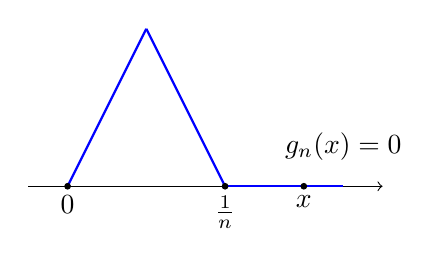
\begin{tikzpicture}
      \draw[->] (-0.5, 0) -- (4, 0);
      \draw[domain=0:1, smooth, variable=\x, blue, thick] plot ({\x}, {2*\x});
      \draw[domain=1:2, smooth, variable=\x, blue, thick] plot ({\x}, {4-2*\x});
      \draw[domain=2:3.5, smooth, variable=\x, blue, thick] plot ({\x}, {0});
      \draw[fill=black] (0, 0) circle (1pt) node[below] {$0$};
      \draw[fill=black] (2, 0) circle (1pt) node[below] {$\frac{1}{n}$};
      \draw[fill=black] (3, 0) circle (1pt) node[below] {$x$};
      \node at (3.5, 0.5) {$g_n(x) = 0$};
    \end{tikzpicture}
  \end{figure}

\item Does $g_n \to 0$ uniformly? No! If possible, this would mean
  \begin{enumerate}
  \item $\sup_{x \in [0, 1]} |g_n(x) - g(x)| \xrightarrow{n \to \infty} 0$;
  \item $\sup_{x \in [0, 1]} |g_n(x)| \geq g_n(\frac{1}{2n}) = 2n \xrightarrow{n \to \infty} \infty$.
  \end{enumerate}
  (a) contradicts (b).

\item
  $$ \int_0^1 g_n(x)dx = 1 \centernot \longrightarrow \int_0^1 g(x)dx = 0. $$
\end{enumerate}

\end{document}
